\documentclass{report}
\usepackage{color,soul}
\usepackage{graphicx}
\usepackage[document]{ragged2e}
\usepackage{subcaption}
\usepackage{wrapfig}
\usepackage{circuitikz}

\usepackage{verbatim}
\title{Computer Studies}
\date{2013-09-01}
\author{Doston Hamrakulov}

\begin{document}
	\maketitle
	\newpage
	\tableofcontents{}
	\newpage
	\chapter{Theoretical part}
	\section{Circuit calculation} 
	
	Calculate the voltages on the resistors shown in the diagram 1. For voltage source V1 use DC
	voltage that is the last three digits of your student ID divided by 10. For example. \textcolor{red}{101REB123}
	means \textcolor{red}{V1 = 12.3 (Volts)}.
	
	\textcolor{red}{R1} is the second digit of the last 3 digits of the student ID + 1. \textcolor{red}{R2} is the last digit of the
	student ID number +1. For example, if your student ID number is \textcolor{red}{101REB123} then \textcolor{red}{R1 = 3},
	‘R2 = 4’.
	Take a picture of the calculation. The calculation process will be required at work \textcolor{red}{P02}.
	Additionally, the calculation will have to be added to the report you will complete at the end of
	the semester\cite{firstRef}
	
	\section{Check modeling with gEDA}
	
	\begin{itemize}
		\item Get into the student’s work area by using ‘ssh’ on a training host with an IP address
		\textcolor{red}{213.175.92.37}. For example: \textcolor{red}{ssh -X x111REB ... @ 213.175.92.37}
		\item Create a folder \underline{‘work’} and go to it. Create a folder \underline{‘P01’} and go to it
		
		\item Launch the program \textcolor{red}{gschem} . Create the schematics shown in the \textbf{\textit{1. }}Select the voltage
		source and resistor values according to the theoretical calculation made at point \textbf{\textit{1.1.}}
		Save the schematics in file called \textcolor{red}{01.sch}. Do not forget to add the ”value” parameter
		to all elements. In addition, there must be a defined ”grounding point”. This is done by
		assigning parameter netname = 0 to one of the connections (nets). See the lecture slides
		for the usage of the program. \cite{firstRef}
		
		\begin{figure}[ht]
			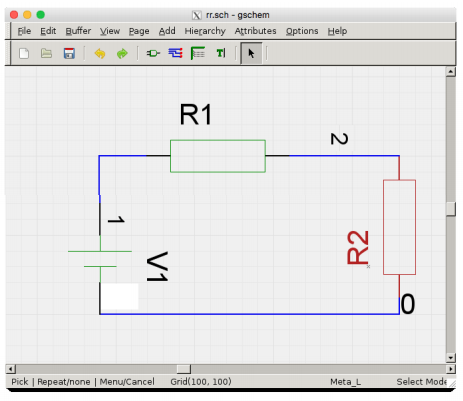
\includegraphics{Figures/one}
			\caption{Shape gschem medium}
			\label{fig:figure1}
		\end{figure}
		
		
		generate the netlist file. For this purpose, run from the command line: \textcolor{red}{gnetlist -g spice 01.sch -o 01.net }.
		\item Using \textcolor{red}{cat} check whether the netlist file has been generated correctly.
		\item Make a simulation of the circuit ‘01.net’ using the program ‘ngspice’. For this purpose,
		run \textcolor{red}{ngspice} from the command line.
		\item Load the created netlist file using the command into ngspice: \textcolor{red}{source 01.net}
		\item Perform a simulation of the transient process (tran) from 0 to 5 seconds in 1 second step.
		\item Use plot to display the signal on the \textbf{\textit{”1”}} connection. Using \textbf{\textit{”hardcopy”}} button save
		the resulting image to ‘011.png’ or make screenshot.
		\item Using plot display the signal in the connection ”2”. Save the resulting image to \textbf{\textit{‘012.png’}}
		or make screenshot. All this will have to be used at work ‘P02’
	\end{itemize}
	
	Bold, Italic, Underline
	Some of the \textbf{greatest}
	discoveries in \underline{science} 
	were made by \textbf{\textit{accident}}
	
	\section{Advanced task: Modeling with QUCS}
	Start simulator QUCS. Locate the ‘Project’ menu, then select ‘Open Project’ point to
	the directory ‘P01’.
	\begin{itemize}
		\item  Choose the tab ‘Components’ on the left. From the palette, select the two components ‘Resistor’ and the source of the component ‘DC Voltage Source’ from the ‘Sources’ menu. Put it all on the work surface as shown in the 2 image. Select the voltage source and resistor values according to the theoretical calculation at point 1.1. Make sure the visible component parameters (R1, R2, V1, etc.) are not overlapped and legible.
		\item  Use CTRL + E to turn on ”wiring” or connection mode and 0connect the components. Do not forget to add ‘Ground’ to the scheme.
	\end{itemize}
	
	
	
	\begin{figure}[t]
		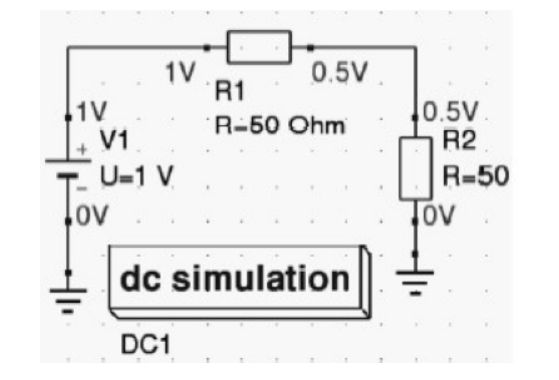
\includegraphics{Figures/Fig}
		\caption{The QUCS schematics environment}
		\label{fig:figure2}
	\end{figure}
	\begin{itemize}
		\item From the menu, open the category ‘simulations’ and add the ”DC simulation” block to
		your schema. Without this block, QUCS will not know what needs to be done.
		\item Save the created scheme with the command sequence File-Save. Name the newly created
		file as ‘02’. Qucs will add the extension (.sch) to the file itself. This will give you the
		file ‘02.sch’.
		
		\item Perform elementary DC mode simulation with the F8 key, which results in calculations
		and determines the voltage on the resistor R2. The simulator variable that derives this
		value is designated R2.V.
		\item Add the schema to the simulation component ‘Parameter sweep’, which is selected from
		the category ‘simulations’ (see Fig. 3). Evaluate the Sweep simulation attributes and
		their parameters displayed on the screen. \cite{firstRef,thirdRef}
		
		
		\begin{figure}[t]
			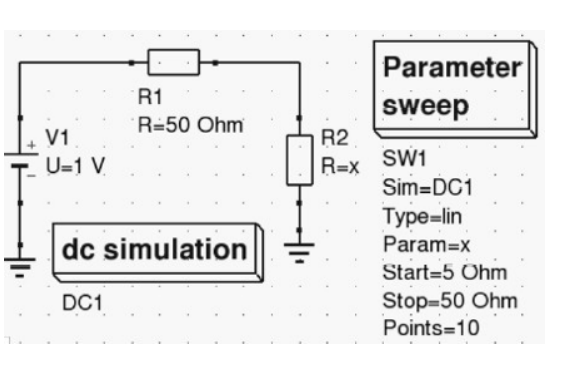
\includegraphics{Figures/Figu}
			\caption{Parameter sweep mode}
			\label{fig:figure3}
		\end{figure}
		
		
		\item Change the value of resistor R2 to the symbol x, which will serve as the argument for the
		current circuit calculation. This symbol: x must also be written in the Param field of the
		component ‘parameter sweep’ attribute field.
		\item Change number of points to 10. Now, simulating parameter x will be changed linearly
		from value 5 Ω to 50Ω at eleven points, where all the parameters of the circuit (current
		and voltages) will be calculated corresponding number of times because they depend of
		resistor R2 value.
		\item Press F8. In the resulting parameter selection form, change them, obtain and estimate
		the calculated voltage value on the resistor R2-UR2, which can be seen in the simulator
		as R2.V.
		\item Enhance the chain by introducing the label for wire connecting R1 to R2. Sometimes it
		says: ”... the node connecting R1 to R2”. Highlight the wire and call it the exit (see Fig. 4). \cite{firstRef}
		
	\end{itemize}
	
	\section{Tabula creation:}
	I have created simple table which is required in practical work:
	
	After that you can use the environment wrapfig, it takes two parameters that are passed inside braces: the alignement that can be l, r, c, i or o; this letters stand for left, right, centre, inner and outer (the last two intended for two-sided documents). The second parameter is the width of the figure, in the example is 0.25 the width of the text. See the reference guide for a list of possible length units.
	
	Then you can use the environment wraptable which takes two parameters: The first one is the alignment that can be l, r, c, i or o for left, right, centre, inner and outer respectively. The second one is the width of the table container, keep in mind that this latter parameter must be the same as the width of the table, otherwise things may not be properly aligned. \cite{firstRef}
	
	
	
	\begin{figure}[b]
		
		
		
		\begin{center}
			\begin{tabular}{ |c|c|c|c| } 
				\hline
				col1 & col2 \\
				\hline
				R1  &  \\ 
				\hline
				R2 &  \\ 
				\hline
				V1 &  \\ 
				\hline
				UR1 &  \\ 
				\hline
				UR2 & \\ 
				\hline
			\end{tabular}
		\end{center}
		\caption{Table}
		\label{tab:table1}
	\end{figure}
	Then you can use the environment wraptable which takes two parameters: The first one is the alignment that can be l, r, c, i or o for left, right, centre, inner and outer respectively. The second one is the width of the table container, keep in mind that this latter parameter must be the same as the width of the table, otherwise things may not be properly aligned.
	Then you can use the environment wraptable which takes two parameters: The first one is the alignment that can be l, r, c, i or o for left, right, centre, inner and outer respectively. The second one is the width of the table container, keep in mind that this latter parameter must be the same as the width of the table, otherwise things may not be properly aligned.
	
	
	
	
	
	
	\section{Circuitikz - for adding the electrical circuit diagram}
	The symbols can also be used along a path, using the transistor-path-syntax(T in front of the
	shape name, see section 6.6). Don´t forget to use parameter n to name the node and get acces to
	the anchors:
	
	

	
	
	
	To then link them up with other components we would use the predefined node anchors. 
	
	For more information about all the components available and how you link components using node anchors, take a look at the documentation.
	
	From the bottom left we have; a resistor, a variable resistor, a transmission line, a closing switch, a european current source, a european voltage source, an empty diode, a full led, a generic bipole and a sinusoidal voltage source.
	
	Bipoles aren’t the only type of component we can use. We can also add in monopoles, tripoles, double bipoles, logic gates and amplifiers. 
	
	
	However we can’t use the ‘to’ keyword to add these in as we’ve done before, because they don’t naturally fit on a single line. Instead we use node notation. For example, this is how we would display an antenna\cite{secondRef,thirdRef}
	
	
	\begin{figure}[b]
		\centering
		\begin{minipage}{.5\textwidth}
			\centering
			\begin{circuitikz} \draw
				(0,2) node[and port] (myand1) {}
				(0,0) node[and port] (myand2) {}
				(2,1) node[xnor port] (myxnor) {}
				(myand1.out) -| (myxnor.in 1)
				(myand2.out) -| (myxnor.in 2);
			\end{circuitikz}
			
			\captionof{figure}{ Logical ports}
			\label{fig:test9}
		\end{minipage}%
		\begin{minipage}{.5\textwidth}
			\centering
			\begin{verbatim}
			\begin{circuitikz} \draw
			(1,0) node[not port] (not1) {}
			(3,0) node[not port] (not2) {}
			(0,0) -- (not1.in)
			(not2.in) -- (not1.out)
			++(0,-1) node[ground] {} to[C] (not1.out)
			(not2.out) -| (4,1) -| (0,0);
			\end{circuitikz}
			\end{verbatim}
			\captionof{figure}{ Logical ports}
			\label{fig:test2}
		\end{minipage}
	\end{figure}
	
	
	From the bottom left we have; a resistor, a variable resistor, a transmission line, a closing switch, a european current source, a european voltage source, an empty diode, a full led, a generic bipole and a sinusoidal voltage source.
	
	Bipoles aren’t the only type of component we can use. We can also add in monopoles, tripoles, double bipoles, logic gates and amplifiers.\cite{firstRef,secondRef}
	
	
	However we can’t use the ‘to’ keyword to add these in as we’ve done before, because they don’t naturally fit on a single line. Instead we use node notation. For example, this is how we would display an antenn
	
	
	\begin{figure}[ht]
		\centering
		\begin{minipage}{.5\textwidth}
			\centering
			\begin{circuitikz} \draw
				(0,0) to[C] (1,0) to[toggle switch , n=Sw] (2.5,0)
				-- (2.5,-1) to[battery1] (1.5,-1) to[R] (0,-1) -| (0,0)
				(Sw.out 2) -| (2.5, 1) to[R] (0,1) -- (0,0);
			\end{circuitikz}
			
			\captionof{figure}{ Logical ports}
			\label{fig:test3}
		\end{minipage}%
		\begin{minipage}{.5\textwidth}
			\centering
			\begin{verbatim}
			\begin{circuitikz} \draw
			(0,0) to[C] (1,0) to[toggle switch , 
			n=Sw] (2.5,0)
			-- (2.5,-1) to[battery1] (1.5,-1)
			to[R] (0,-1) -| (0,0)
			(Sw.out 2) -| (2.5, 1) to[R] (0,1) 
			-- (0,0);
			\end{circuitikz}
			\end{verbatim}
			\captionof{figure}{ Logical ports}
			\label{fig:test14}
		\end{minipage}
	\end{figure}
	
	
	\subsection{More circuit diagrams}
	
	\begin{figure}[ht]
		
		\begin{minipage}{.5\textwidth}
			
			\begin{circuitikz} 
				\draw
				(0,0) node[op amp] (opamp) {}
				(opamp.+) node[left] {$v_+$}
				(opamp.-) node[left] {$v_-$}
				(opamp.out) node[right] {$v_o$}
				(opamp.up) --++(0,0.5) node[vcc]{5\,\textnormal{V}}
				(opamp.down) --++(0,-0.5) node[vee]{-5\,\textnormal{V
					}};
				\end{circuitikz}
				
				\captionof{figure}{ Logical ports}
				\label{fig:test11}
			\end{minipage}%
			\begin{minipage}{.5\textwidth}
				
				
				\begin{circuitikz} \draw
					(0,0) node[transformer] (T) {}
					(T.A1) node[anchor=east] {A1}
					(T.A2) node[anchor=east] {A2}
					(T.B1) node[anchor=west] {B1}
					(T.B2) node[anchor=west] {B2}
					(T.base) node{K};
				\end{circuitikz}
				
				\captionof{figure}{ Logical ports}
				\label{fig:test4}
			\end{minipage}
		\end{figure}
		
		
		For more information about all the components available and how you link components using node anchors, take a look at the documentation. From the bottom left we have; a resistor, a variable resistor, a transmission line, a closing switch, a european current source, a european voltage source, an empty diode, a full led, a generic bipole and a sinusoidal voltage source. Bipoles aren’t the only type of component we can use. We can also add in monopoles, tripoles, double bipoles, logic gates and amplifiers. However we can’t use the ‘to’ keyword to add these in as we’ve done before, because they don’t naturally fit on a single line. Instead we use node notation. For example, this is how we would display an antenna \cite{secondRef}
		
		
		
		
		\chapter{Practical part}
		\section{Work with GEDA programs} 
		\subsection{Work with gschem}
		After that you can use the environment wrapfig, it takes two parameters that are passed inside braces: the alignement that can be l, r, c, i or o; this letters stand for left, right, centre, inner and outer (the last two intended for two-sided documents). The second parameter is the width of the figure, in the example is 0.25 the width of the text. See the reference guide for a list of possible length units.
		After that you can use the environment wrapfig, it takes two parameters that are passed inside braces: the alignement that can be l, r, c, i or o; this letters stand for left, right, centre, inner and outer (the last two intended for two-sided documents). The second parameter is the width of the figure, in the example is 0.25 the width of the text. See the reference guide for a list of possible length units.
		
		
		\begin{figure}[b]
			\centering
			\begin{minipage}{.5\textwidth}
				\centering
				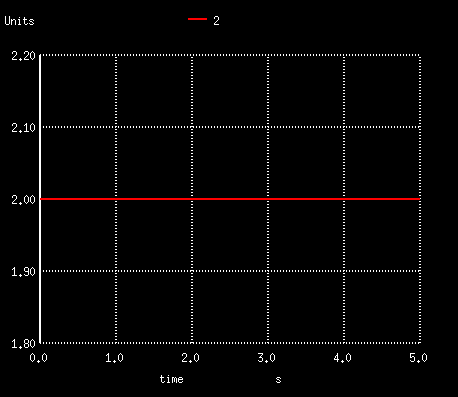
\includegraphics[width=.4\linewidth]{Figures/oneFig.png}
				\captionof{figure}{Gschem}
				\label{fig:test8}
			\end{minipage}%
			\begin{minipage}{.5\textwidth}
				\centering
				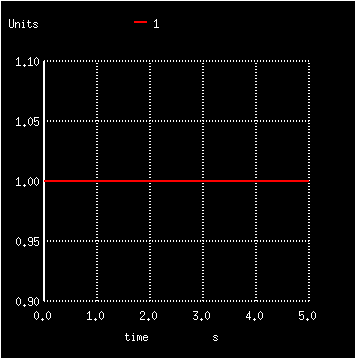
\includegraphics[width=.4\linewidth]{Figures/twoFig.png}
				\captionof{figure}{Gschem graph}
				\label{fig:test7}
			\end{minipage}
		\end{figure}
		
		
		
		
		
		After that you can use the environment wrapfig, it takes two parameters that are passed inside braces: the alignement that can be l, r, c, i or o; this letters stand for left, right, centre, inner and outer (the last two intended for two-sided documents). The second parameter is the width of the figure, in the example is 0.25 the width of the text. See the reference guide for a list of possible length units.
		After that you can use the environment wrapfig, it takes two parameters that are passed inside braces: the alignement that can be l, r, c, i or o; this letters stand for left, right, centre, inner and outer (the last two intended for two-sided documents). The second parameter is the width of the figure, in the example is 0.25 the width of the text. See the reference guide for a list of possible length units.
		After that you can use the environment wrapfig, it takes two parameters that are passed inside braces: the alignement that can be l, r, c, i or o; this letters stand for left, right, centre, inner and outer (the last two intended for two-sided documents). The second parameter is the width of the figure, in the example is 0.25 the width of the text. See the reference guide for a list of possible length units. \cite{firstRef,thirdRef}
		
		
		
		
		\subsection{ Work with gnetlist}
		
		\verbatiminput{01.net}
		
		\subsection{Work with ngspice’}
		After that you can use the environment wrapfig, it takes two parameters that are passed inside braces: the alignement that can be l, r, c, i or o; this letters stand for left, right, centre, inner and outer (the last two intended for two-sided documents). The second parameter is the width of the figure, in the example is 0.25 the width of the text. See the reference guide for a list of possible length units.
		After that you can use the environment wrapfig, it takes two parameters that are passed inside braces: the alignement that can be l, r, c, i or o; this letters stand for left, right, centre, inner and outer (the last two intended for two-sided documents). The second parameter is the width of the figure, in the example is 0.25 the width of the text. See the reference guide for a list of possible length units. \cite{firstRef,thirdRef}
		
		\begin{figure}[ht]
			\centering
			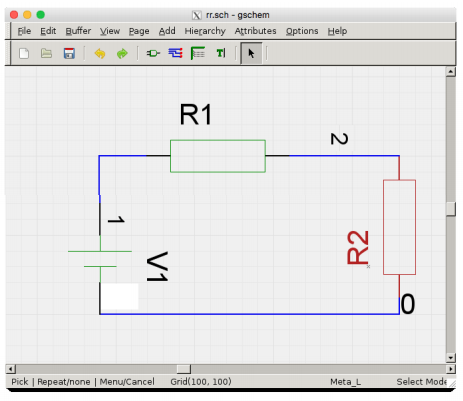
\includegraphics[width=0.6\linewidth]{Figures/one} 
			\caption{Plots from the simulations of voltage on R1 and R2}
			\label{fig:figure5}
		\end{figure}
		
		
		
		
		After that you can use the environment wrapfig, it takes two parameters that are passed inside braces: the alignement that can be l, r, c, i or o; this letters stand for left, right, centre, inner and outer (the last two intended for two-sided documents). The second parameter is the width of the figure, in the example is 0.25 the width of the text. See the reference guide for a list of possible length units.
		After that you can use the environment wrapfig, it takes two parameters that are passed inside braces: the alignement that can be l, r, c, i or o; this letters stand for left, right, centre, inner and outer (the last two intended for two-sided documents). The second parameter is the width of the figure, in the example is 0.25 the width of the text. See the reference guide for a list of possible length units.\cite{firstRef,thirdRef}
		
		After that you can use the environment wrapfig, it takes two parameters that are passed inside braces: the alignement that can be l, r, c, i or o; this letters stand for left, right, centre, inner and outer (the last two intended for two-sided documents). The second parameter is the width of the figure, in the example is 0.25 the width of the text. See the reference guide for a list of possible length units.\cite{firstRef,thirdRef}
		
		After that you can use the environment wrapfig, it takes two parameters that are passed inside braces: the alignement that can be l, r, c, i or o; this letters stand for left, right, centre, inner and outer (the last two intended for two-sided documents). The second parameter is the width of the figure, in the example is 0.25 the width of the text. See the reference guide for a list of possible length units.\cite{firstRef,thirdRef}
		
		
		\section{Work with QUCS programs}
		
		
		\begin{itemize}
			\item Image of the schematics
			\item Plot (curve) of DC simulation.
			\item Curve from Sweep simulation (advanced topic).
			\item Sweep simulation table (advanced topic).
			\item Explanations for each image and table (advanced topic).
		\end{itemize}
		
		
		
		
		\begin{thebibliography}{9}
			\bibitem{firstRef} 
			Documentation of ShareLetatex, Online
			\textit{The \LaTeX\ Companion}. 
			Addison-Wesley, Reading, Massachusetts, 2003.
			
			\bibitem{secondRef} 
			Massimo A. Redaelli (m.redaelli@gmail.com)
			\textit{CircuiTikZ}. (German) 
			[\textit{On the electrodynamics of moving bodies}]. 
			Annalen der Physik, 322(10):891–921, 2006.
			
			\bibitem{thirdRef} 
			Latex Tutorial Online
			\textit{http://www.latex-tutorial.com/tutorials}
		\end{thebibliography}
		
	\end{document}